% From Video to Digital Twin: Accelerating Spatial Twins with World Models and NVIDIA Omniverse
% Built on the Research Future LaTeX template supplied by the author. Build: see paper/README.md.
%
% Drafting rule for this file: every number that has not been measured on a real
% run is a \TBD{} placeholder. Do not replace a placeholder with an estimate.
\documentclass{article}
\usepackage[utf8]{inputenc}
\usepackage{authblk}
\usepackage{setspace}
\usepackage[margin=1.25in]{geometry}
\usepackage{graphicx}
\graphicspath{ {./figures/} }
\usepackage{subcaption}
\usepackage{amsmath}
\usepackage{lineno}
\linenumbers

% Additions to the template: tables, the architecture diagram, colored placeholders, links.
\usepackage{booktabs}
\usepackage{array}
\usepackage{tabularx}
\usepackage{xcolor}
\usepackage{tikz}
\usetikzlibrary{arrows.meta,positioning,fit,backgrounds}
\usepackage[hidelinks]{hyperref}
\setlength{\emergencystretch}{2em}

% \TBD{...}: a value or passage that needs a real measurement or decision.
% Change \drafttrue to \draftfalse to check that none remain (the build then stops at any \TBD).
\newif\ifdraft
\drafttrue
\ifdraft
  \newcommand{\TBD}[1]{\textcolor{red!70!black}{\textbf{[TBD: #1]}}}
\else
  \newcommand{\TBD}[1]{\errmessage{Unresolved TBD: #1}}
\fi
\newcommand{\figplaceholder}[2]{%
  \fbox{\parbox[c][#1][c]{0.95\linewidth}{\centering\small\textcolor{red!70!black}{\textbf{[FIGURE TBD]} #2}}}}
\newcommand{\code}[1]{\texttt{\small #1}}

%%%%%% Bibliography %%%%%%
\usepackage[style=nejm,
citestyle=numeric-comp,
sorting=none,
backend=bibtex]{biblatex}
\addbibresource{refs.bib}

%%%%%% Title %%%%%%
\title{From Video to Digital Twin: Accelerating Spatial Twins with World Models and NVIDIA Omniverse}

%%%%%% Authors %%%%%%
\author[1*]{Somesh Mohapatra}

%%%%%% Affiliations %%%%%%
\affil[1]{Independent Researcher.}
\affil[*]{Address correspondence to: pikulsomesh@gmail.com}

%%%%%% Date %%%%%%
\date{}

%%%%%% Spacing %%%%%%
\onehalfspacing

\begin{document}

\maketitle

%%%%%% Abstract %%%%%%
\begin{abstract}
Digital twins, virtual copies of a site kept in sync with its live data, help
warehouses plan layouts and catch failures, but building one
usually takes laser scans, hand-drawn 3D models and simulation specialists,
which puts twins out of reach for most non-profits. We asked whether an
ordinary walkthrough video is enough to start one, and built an open pipeline
in three steps. First, a world model, an AI system that infers the 3D structure
of a scene from a few images and can generate views the camera never captured,
estimates camera positions and real-world depth for a handful of frames, which
are fused into a 3D Gaussian-splat scene. Second,
the scene is connected to operational data, such as freezer temperatures and
forklift positions, through a serverless backend on Amazon Web Services that
costs nothing when idle. Third, NVIDIA Omniverse displays the twin with its
live data, with a web browser and Blender as alternatives. Universal Scene
Description, an open 3D file standard that now stores Gaussian splats natively,
is the only interface between the steps. Applied to three areas of a food bank
from a public news video, twenty frames produced a twin of about 747,000 splats
in one 48.5-megabyte file for 200 world-model credits (20 US cents), plus up to
800 more if two failed requests are billed. Generating views of unfilmed areas
failed on the provider's side both times, so the twin shows only what the
camera saw. A conventional splat model trained locally from 72
frames of the same video, at no credit cost, made one area photorealistic near
the filmed path. Cloud cost is \TBD{pending AWS deployment}. A phone video and
a world model can bring a first facility twin within reach of charitable
organizations; filling in unseen space is the open step.
\end{abstract}

%%%%%% Main Text %%%%%%

\section{Introduction}
A digital twin is a virtual representation of a physical asset that stays
synchronized with it through data \cite{grieves2017digital,kritzinger2018digital}.
In industry, twins are used to plan layouts, monitor equipment and rehearse
changes before they are made on the floor \cite{tao2019digital,fuller2020digital}.
The geometry of a facility twin is usually the expensive part. It comes from
terrestrial laser scanning, photogrammetry campaigns or hand-built
computer-aided design (CAD) models, and specialists then import it into a
simulation tool. That cost is tolerable for an automotive plant. It is
prohibitive for a regional food bank, which runs warehouse-scale cold-chain
logistics on a non-profit budget.

Two developments change that cost structure. Neural scene representations,
and 3D Gaussian Splatting in particular \cite{kerbl20233d}, produce
photorealistic scenes that render in real time from ordinary images. Classical
reconstruction recovers camera poses with structure-from-motion
\cite{schoenberger2016sfm}; neural radiance fields \cite{mildenhall2020nerf}
improved view synthesis but render slowly; learned multi-view geometry such as
DUSt3R \cite{wang2024dust3r} reduces the number of views needed. All of these
reconstruct only what was observed. Generative world models
\cite{ha2018world,brooks2024video} go further: from a few views they produce a
coherent, explorable 3D world and fill in regions the input never covered.
World Labs' Marble \cite{worldlabs_marble} exposes this capability through an
API that returns Gaussian-splat worlds. For a twin, generation has a double
edge. It makes a sparse walkthrough usable, but it also invents geometry.

In parallel, Universal Scene Description (OpenUSD), originally from Pixar and
now developed under the Alliance for OpenUSD, has become an open,
vendor-neutral scene description with layered composition and typed schemas
\cite{openusd}. Its 26.03 release added the
\code{ParticleField3DGaussianSplat} schema family
\cite{aousd2603,usd_gsplat_schema}, so a splat reconstruction is no longer a
viewer-specific file. It can sit in the same stage as sensors, equipment and
annotations. NVIDIA Omniverse \cite{omniverse} is a USD-native platform for
real-time RTX rendering and simulation. Its licensing is mixed: some
components are open source, while the Kit SDK is distributed under NVIDIA's
own license terms: the Kit App Template states that its software and materials
are governed by the NVIDIA Software License Agreement and the Product-Specific
Terms for NVIDIA Omniverse \cite{kit_app_template}, not an open-source
license.

Surveys of digital twins identify geometry acquisition, data integration and
interoperability as the recurring barriers \cite{tao2019digital,fuller2020digital}.
This work addresses the first and third barriers directly and keeps the second
deliberately thin. We ask whether these pieces can be composed into a twin that
a small team can build from a phone video, quickly and at very low cost. Our
answer is a three-step pipeline (Figure~\ref{fig:overview}):
\begin{enumerate}
  \item \textbf{Video to digital twin with world models.} Blur-aware frame
        extraction feeds a world model that returns a Gaussian-splat world,
        which is converted to an OpenUSD stage in metric, Y-up coordinates.
  \item \textbf{Connecting existing data systems on Amazon Web Services (AWS).}
        A serverless API exposes operational data in the twin's coordinate
        frame through a small, versioned JSON contract. The reference
        implementation simulates cold-chain telemetry; the contract is
        designed so that a real sensor feed or warehouse management system
        can replace the simulator without changing any renderer.
  \item \textbf{NVIDIA Omniverse as the visualization layer.} Omniverse
        renders the USD twin with live data bound to scene objects. A
        browser viewer and Blender read the same USD and the same JSON, so
        the renderer is a deployment choice rather than an architectural one.
\end{enumerate}

The contributions are an open-source pipeline from walkthrough video to an
Omniverse-ready OpenUSD Gaussian-splat twin, including the coordinate and
packaging corrections needed to make world-model output a valid metric USD
asset; an architecture in which OpenUSD and a small telemetry contract are the
only interfaces between reconstruction, data and rendering, with a serverless
backend that has no standing cost; an operations layer that models
inventory, flows, docks and a community kitchen behind the same API and as
OpenUSD prims; cost controls that make paid world-model generation safe to
run unattended; and a Tech-for-Good case study of a food
bank, with an account of what the world model recovered, what it was asked
to invent and where that step failed. Food banks are logistics operations: when
the Central Texas Food Bank moved into its 135,000-square-foot Austin
facility in 2016, the new building held seven times the refrigeration and
freezer capacity of the old one \cite{ctfb2016facility}, and its newer Waco
hub combines a warehouse and distribution hub, a kitchen, a food market and a
training center in 64,000 square feet \cite{kxxv2026waco}. Cold storage at that
scale is exactly what a twin with live temperatures is meant to watch.

\section{Results}

\subsection{Three steps joined by one open contract}
The steps share data, not code. Two artifacts cross step boundaries
(Table~\ref{tab:contracts}). The reconstruction step publishes a USD package,
the SPZ splat file it was converted from (for lightweight viewers) and a
metadata file recording scale, ground offset and provenance. The data step
publishes a JSON document whose positions are in meters in the same frame as
the USD stage. A renderer needs nothing else, which is what lets Omniverse, a
browser and Blender coexist (Figure~\ref{fig:overview}).

\begin{figure}[t]
\centering
\begin{tikzpicture}[
  box/.style={draw, rounded corners=2pt, align=center, font=\small, minimum height=1.3cm, text width=2.85cm, fill=white},
  lay/.style={draw=black!25, rounded corners=4pt, inner xsep=6pt, inner ysep=5pt, fill=black!4},
  lbl/.style={font=\footnotesize\bfseries, anchor=south west, inner sep=1pt},
  arr/.style={-{Stealth[length=2.2mm]}, thick},
  node distance=0.9cm and 0.45cm]
  % Step 1
  \node[box] (vid) {Walkthrough video\\\footnotesize MP4 or phone};
  \node[box, right=of vid] (frm) {Blur-aware frames\\\footnotesize ffmpeg, $\le$40};
  \node[box, right=of frm] (wm) {World model\\\footnotesize Gaussian-splat world};
  \node[box, right=of wm] (usd) {OpenUSD stage\\\footnotesize metric, Y-up};
  \node[lbl] at ([yshift=3pt]vid.north west) (l1) {Step 1: video $\rightarrow$ twin with a world model};
  \draw[arr] (vid) -- (frm); \draw[arr] (frm) -- (wm); \draw[arr] (wm) -- (usd);
  % Step 2 (columns 1-3, leaving column 4 free for the USD arrow)
  \node[box, below=1.25cm of vid] (src) {Existing systems\\\footnotesize IoT, WMS, cold chain};
  \node[box, right=of src] (api) {Serverless API\\\footnotesize Lambda + HTTP API};
  \node[box, right=of api] (json) {Telemetry JSON\\\footnotesize meters, twin frame};
  \node[lbl] at ([yshift=3pt]src.north west) (l2) {Step 2: existing data on AWS};
  \draw[arr] (src) -- (api); \draw[arr] (api) -- (json);
  % contract bar
  \coordinate (barl) at ([yshift=-1.1cm]src.south -| vid.west);
  \coordinate (barr) at ([yshift=-1.1cm]src.south -| usd.east);
  \node[draw, thick, rounded corners=2pt, fill=blue!6, fit=(barl)(barr), inner xsep=0pt, inner ysep=0.35cm,
        label={[font=\small]center:Open contract: OpenUSD splat stage, SPZ and metadata, plus the telemetry JSON}] (bar) {};
  \draw[arr] (usd.south) -- (usd.south |- bar.north);
  \draw[arr] (json.south) -- (json.south |- bar.north);
  % Step 3
  \node[box, below=0.9cm of bar.south, anchor=north] (ov) {NVIDIA Omniverse\\\footnotesize RTX + live-data extension};
  \node[box, left=of ov] (web) {Browser\\\footnotesize Spark on SPZ};
  \node[box, right=of ov] (bl) {Blender\\\footnotesize alternative};
  \node[lbl, anchor=north west] at ([yshift=-3pt]web.south west) (l3) {Step 3: visualization};
  \foreach \n in {web,ov,bl} \draw[arr] (bar.south -| \n.north) -- (\n.north);
  \begin{scope}[on background layer]
    \node[lay, fit=(l1)(vid)(usd)] {};
    \node[lay, fit=(l2)(src)(json)] {};
    \node[lay, fit=(l3)(web)(bl)] {};
  \end{scope}
\end{tikzpicture}

\caption{The Auto-Twin pipeline. The open contract is the only
interface between steps: the OpenUSD stage (with the SPZ it was converted from
and a metadata file) and the telemetry JSON. Any box can be replaced without
changing the others.}
\label{fig:overview}
\end{figure}

\begin{table}[t]
\caption{Contracts between the pipeline's steps. Changes to the telemetry contract are additive only.}
\centering\small
\begin{tabularx}{\linewidth}{@{}l>{\raggedright\arraybackslash}p{3.6cm}>{\raggedright\arraybackslash}X@{}}
\toprule
Boundary & Artifact & Rules \\
\midrule
1 to 3 & \code{factory.usdz}, \code{factory.spz}, \code{factory.meta.json} &
  Metric (\code{metersPerUnit}\,=\,1), Y-up, ground at $y=0$; alignment and provenance in the metadata file. \\
2 to 3 & \code{GET /telemetry} (JSON) &
  \code{zones[]} (temperature, setpoint, humidity, door, status, position) and
  \code{forklifts[]} (position, heading, speed, battery); positions in meters in the twin frame; \code{simulated} flag. \\
\bottomrule
\end{tabularx}
\label{tab:contracts}
\end{table}

\subsection{A walkthrough news video yields usable input for three zones}
The input was a public news walkthrough of a new Central Texas Food Bank
facility, which by its broadcaster and on-screen campaign appears to be the
Waco hub \cite{kxxv2026waco} (18\,min\,32\,s, 1920\,$\times$\,1080 at 59.94 frames per second)
\cite{kxxv2026ctfb}. Two people appear in almost every shot and a lower-third
graphic is burned into each frame, which makes it a realistic rather than a
curated input. A multi-image world needs overlapping views of one space, so we
targeted a single zone. Surveying the video at one frame every 10\,s gave the
candidate zones in Table~\ref{tab:zones}. The pallet-racking aisle was
captured first, because the camera circles one bay and then looks down the
aisle, and because it is the zone that matters most for inventory locations,
forklift paths and telemetry. The volunteer sorting room and the client market
were captured in a second run, from narrower windows in which the camera moves
enough to give overlapping views. The layout of the twin is inspired by the Central Texas Food Bank;
it is not an exact replica, and the world model adds plausible operational
areas that the source video does not show.

\begin{table}[t]
\caption{Candidate zones in the source walkthrough and the assessment that led to the three captured zones.}
\centering\small
\begin{tabularx}{\linewidth}{@{}llX@{}}
\toprule
Time (min:s) & Zone & Assessment \\
\midrule
0:45--1:35 & Volunteer sorting room & Captured from 0:48--1:06, where the camera moves; 6 frames. \\
2:10--2:50 & Freezer and cooler doors & Mostly blank walls; fogged at 2:40. \\
5:05--6:00 & Loading dock & People fill the frame. \\
6:10--7:45 & Pallet-racking aisle & Captured. Racking, wrapped pallets and a pallet jack; the camera circles a bay and looks down the aisle; one view has no people; 8 frames. \\
9:20--10:00 & Client grocery market & Captured from 9:16--9:50; people block the center and were masked; 6 frames. \\
13:50--16:40 & Commercial kitchen & Reflective stainless steel, hard for splats. \\
\bottomrule
\end{tabularx}
\label{tab:zones}
\end{table}

Automatic frame selection failed on this footage. Ranking frames by variance
of the Laplacian, a standard sharpness score, rewards in-focus faces, and on
this video it selected six near-identical shots of the presenters. The eight
inputs were therefore chosen by hand for viewpoint spread and absence of
people, spanning 6:13 to 7:33 (Figure~\ref{fig:inputs}): three views of one bay
from different angles, one view with no people, two from the opposite side of
the aisle, a wide shot under the beam and one looking down the main aisle
toward the dock. The sorting room and market inputs, six frames each, were
picked by hand in the same way from 40 extracted frames per zone. In every
input, the two presenters were covered by hand-drawn boxes that exclude those
pixels from reconstruction.

\begin{figure}[t]
\centering
\IfFileExists{figures/contact_sheet.jpg}{%
  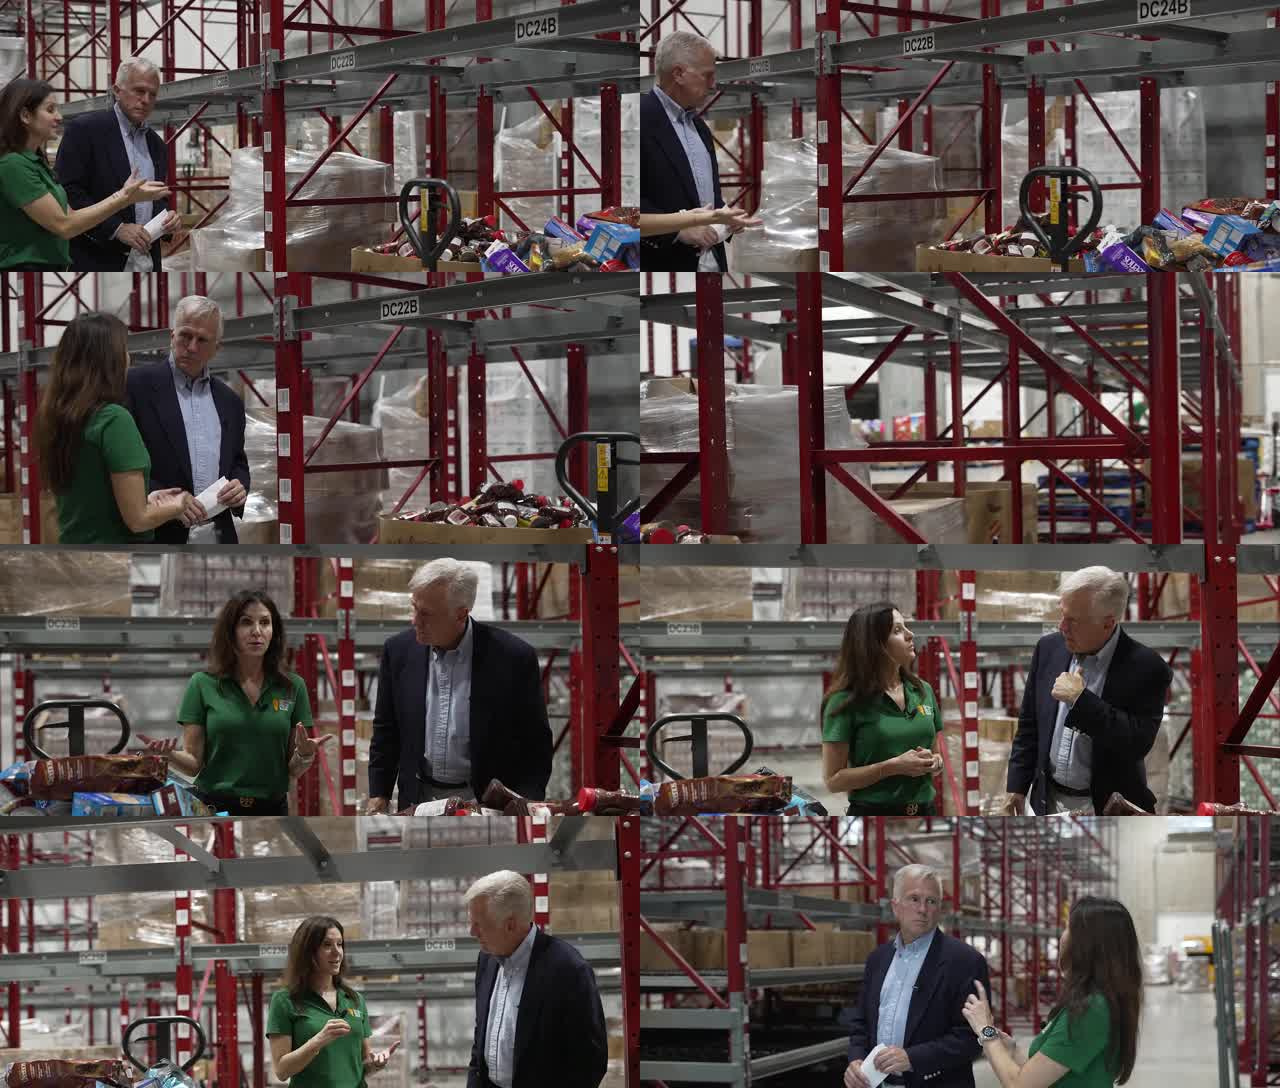
\includegraphics[width=\linewidth]{contact_sheet.jpg}}{%
  \figplaceholder{4cm}{Contact sheet of the eight input frames.}}
\caption{The eight input frames from the racking aisle, 1920\,$\times$\,816
pixels after cropping the broadcast graphic. The sorting room and market
inputs are in the repository.}
\label{fig:inputs}
\end{figure}

\subsection{The world model recovers metric geometry, but did not yet extrapolate}
The world model posed every input frame and returned metric depth with a
per-pixel confidence. The depth is plausible at real scale: in the racking
aisle, the first beam lands about 0.4\,m above the camera, consistent with a
beam about 1.9\,m above the floor for a handheld camera. Fusing the posed
frames gave 270{,}423 splats for the racking aisle, about 282{,}000 for the
sorting room (keeping every third pixel) and about 195{,}000 for the client
market, about 747{,}000 in total (Table~\ref{tab:results}). The floor was found from a dense horizontal
slab of points in the sorting room and from the world model's own ground plane
in the market; in the racking aisle, where the floor is barely visible, it was
placed 1.5\,m below the source cameras.

The generative step did not succeed. Both requests to generate a ring of eight
new views around the racking aisle returned \code{EXECUTION\_FAILED} without
further detail: the first placed every target camera at one center, the
second spread them on a 0.6\,m ring and centered the context principal points.
Retries were paused until it is known whether failed requests are billed. The
twin therefore covers only what the camera saw (Figure~\ref{fig:results}):
each zone is a partial shell seen from its source viewpoints, with gaps where
the presenters were masked and where the camera never pointed. These gaps are
exactly where generated views are meant to go.

\begin{figure}[t]
\centering
\begin{subfigure}{0.49\textwidth}
  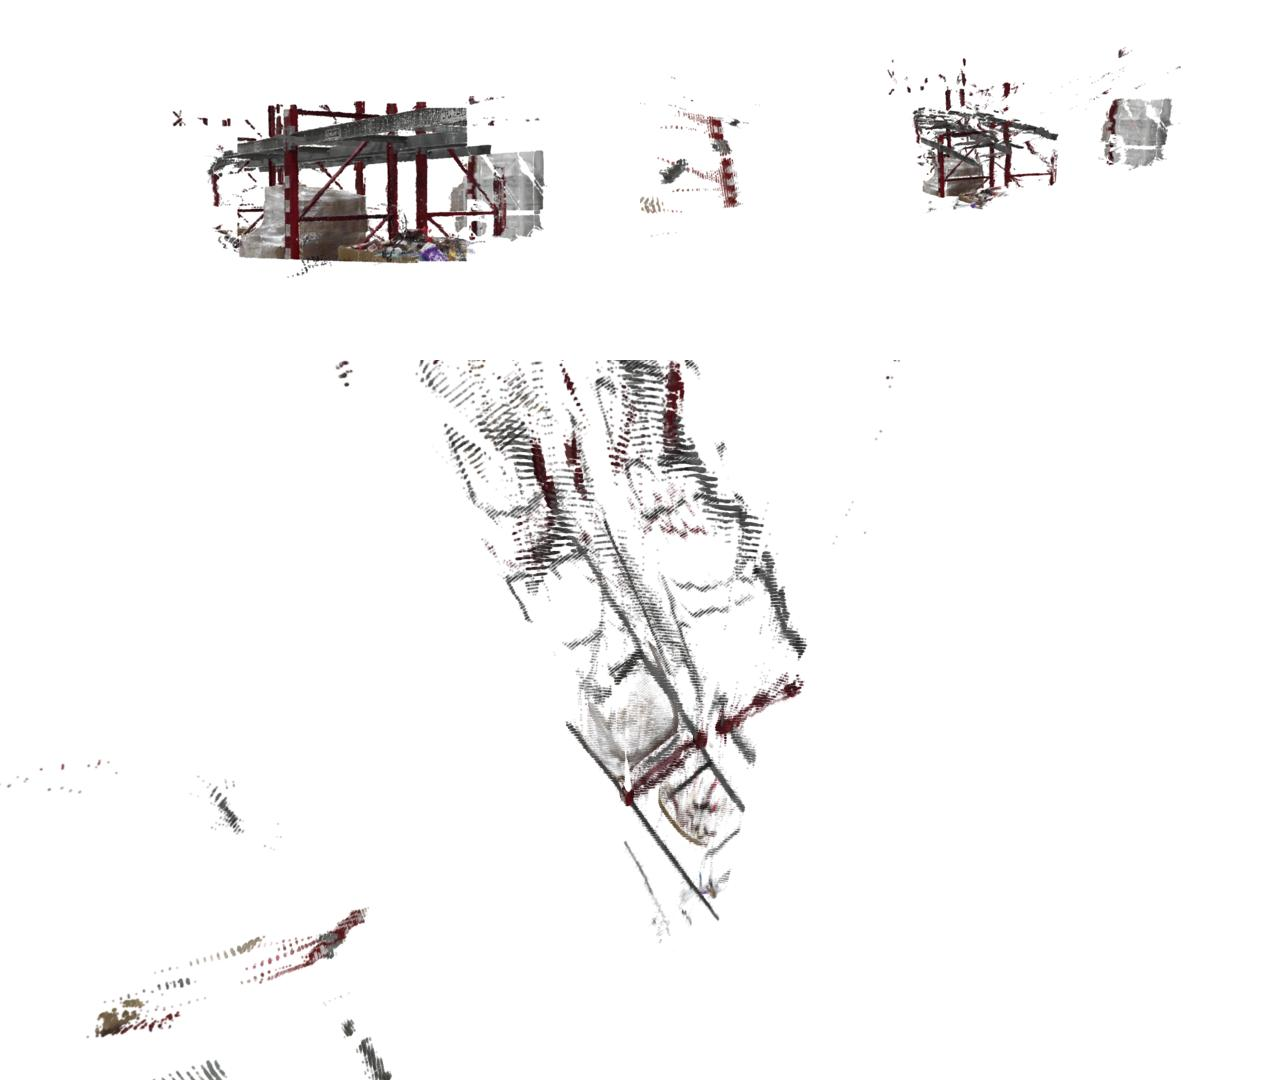
\includegraphics[width=\linewidth]{racking_preview.jpg}
  \caption{\label{fig:resultsA}}
\end{subfigure}\hfill
\begin{subfigure}{0.49\textwidth}
  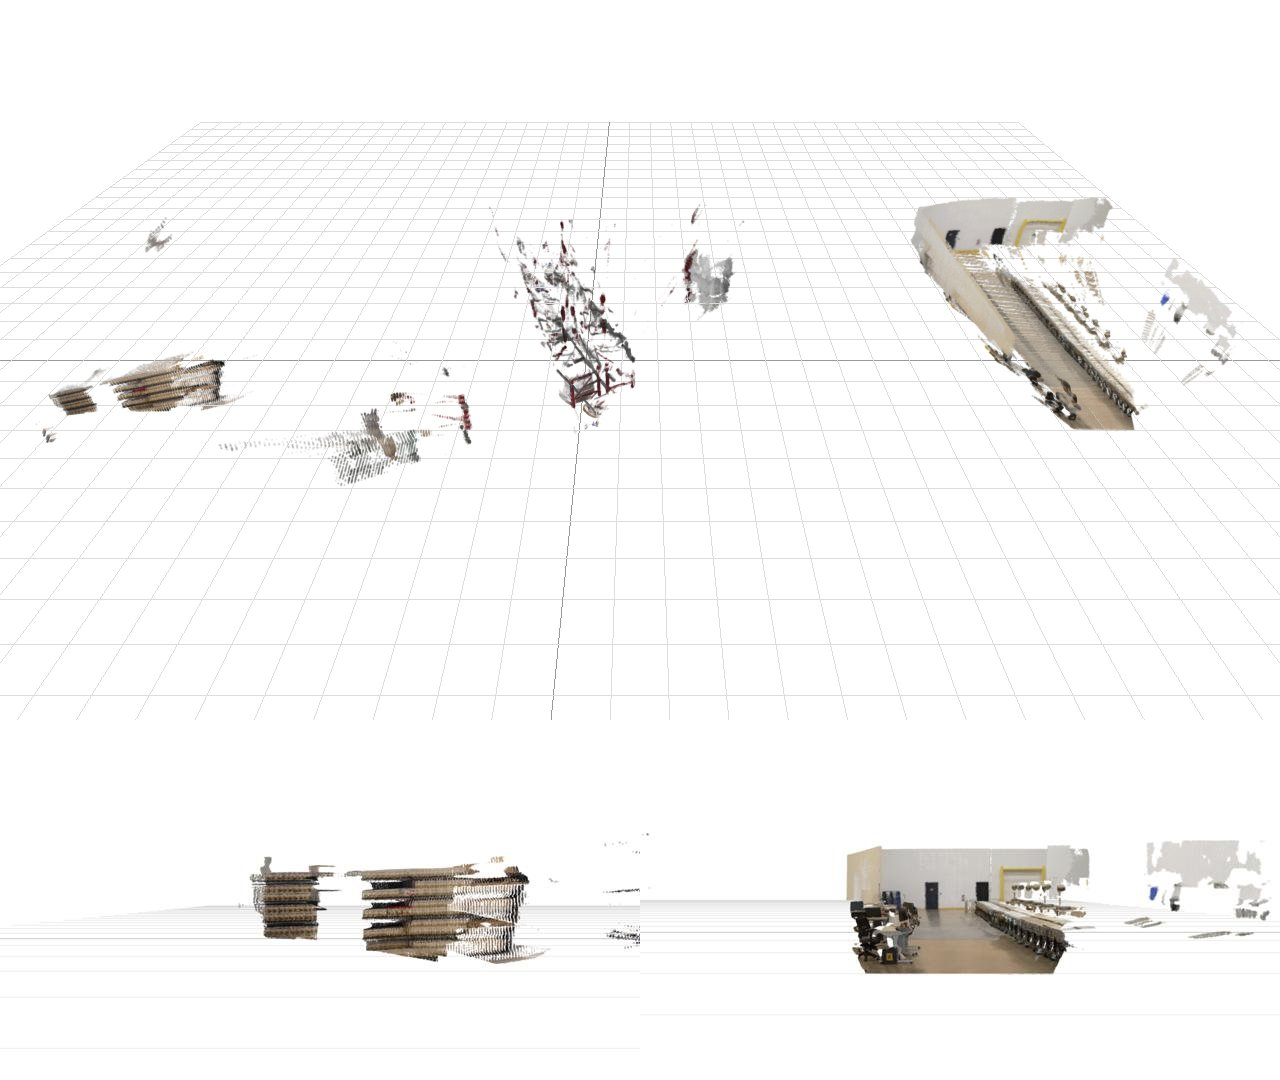
\includegraphics[width=\linewidth]{site_preview.jpg}
  \caption{\label{fig:resultsB}}
\end{subfigure}
\caption{The fused twin rendered in Spark 0.1.10. (\subref{fig:resultsA}) The
racking aisle from two viewpoints: red racking, a wrapped pallet and the
donation bin are recovered where the camera looked, and the rest of the aisle
is empty. (\subref{fig:resultsB}) Top: the three zones placed on one site plan
on a 1\,m grid; bottom: the market and the sorting room from their source
viewpoints. No generated views are included.}
\label{fig:results}
\end{figure}

\subsection{Locally trained splats make one zone photorealistic at no credit cost}
To separate what the world model contributes from what Gaussian splatting
contributes, the racking aisle was also reconstructed the conventional way,
without any paid call. A 100\,s segment of the tour (from 6:08) was sampled at
4 frames per second and 960 pixels wide; people were masked automatically,
together with the broadcast graphic; and sharp frames in which the camera had
moved were kept, leaving 72 frames, nine times as many as the world-model
capture used. Camera poses came from structure-from-motion on the CPU
\cite{schoenberger2016sfm,colmap}, and a 3D Gaussian Splatting model
\cite{kerbl20233d} was trained on the CPU with a trainer written for this work.
The exported zone holds 181{,}556 splats spanning about
28\,$\times$\,9\,$\times$\,33\,m, in a 2.9\,MB SPZ file and an 11.9\,MB USDZ
package with the same contract as the world-model zones, and cost 0 credits.
Near the filmed path, the racking, wrapped pallets, shelf labels and the bottle
bin read photographically, where the world-model capture shows sparse
fragments (Figure~\ref{fig:photoreal}). Two trade-offs remain. Structure from
motion has no metric scale, so the scene was scaled by assuming the camera was
held 1.6\,m above the floor, where the world model measured depth directly
from eight frames. And the areas behind the presenters, who stand in the same
place through most of the segment, were never filmed and train to a soft grey
fill. \TBD{training steps and wall-clock time for the racking zone; results for
the sorting room and market}.

\begin{figure}[t]
\centering
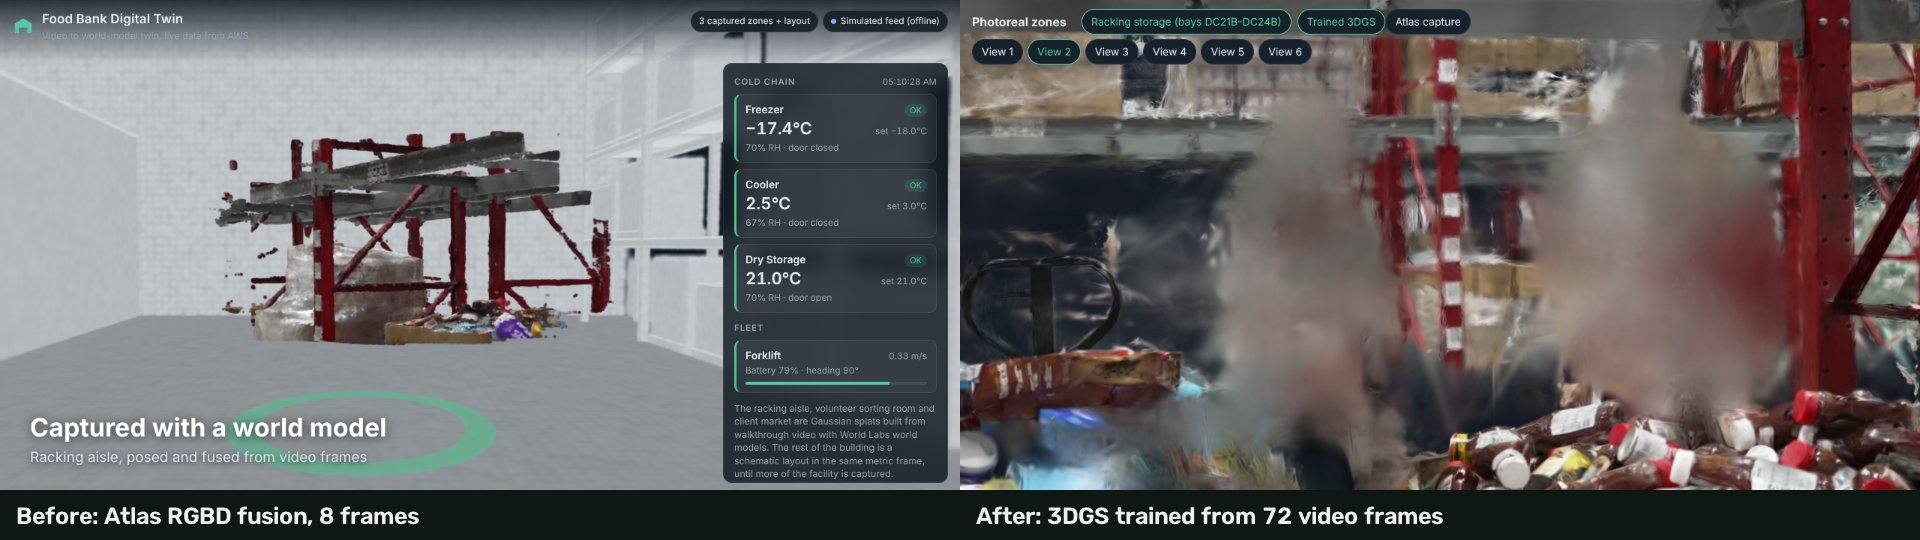
\includegraphics[width=\linewidth]{photoreal_before_after.jpg}
\caption{The racking aisle in the browser viewer. Left: the world-model capture,
posed and fused from 8 frames. Right: a 3D Gaussian Splatting model trained
locally from 72 frames of the same video, from a source camera. The grey haze
on the right is where the masked presenters stood.}
\label{fig:photoreal}
\end{figure}

\subsection{World-model output becomes a valid, metric OpenUSD asset}
Converting the splat world to OpenUSD required four corrections, described in
Materials and Methods: a coordinate transform from the world model's camera
frame, an untyped reference prim so the splat schema is not hidden, binary
packaging with correct alignment, and a choice of splat density by target.
After conversion the pipeline re-opens the package and fails unless it finds
a \code{ParticleField3DGaussianSplat} prim with positions. In a synthetic test
with 20{,}000 splats at spherical-harmonic degree 1, the SPZ file was 262\,KB
and the USDZ package 2.0\,MB, a 7.7-fold increase, because SPZ is quantized
and compressed while USD stores 32-bit floats and USDZ is uncompressed by
specification. For the racking aisle, the 270{,}423-splat SPZ file (spherical
harmonics of degree 0) is 2.1\,MB and its USDZ package 17.5\,MB, an 8.5-fold
increase. The three zones are composed into one stage, \code{/World/Site}, in
which each zone is a separately referenced layer with its own placement, so a
zone can be re-captured without touching the others; the packaged site is
48.5\,MB for about 747{,}000 splats.

\subsection{Live data reaches the twin at near-zero standing cost}
The reference backend serves simulated cold-chain telemetry for three zones
(freezer, cooler and dry storage, with setpoints of $-18^\circ$C, $3^\circ$C
and $21^\circ$C) and one forklift on a closed path from the dock through the
storage aisles. It has no virtual private cloud, NAT gateway, database or
provisioned capacity, so an idle twin costs nothing beyond storage.
No real data connector is deployed yet, so all telemetry in this paper is
simulated. \TBD{pending AWS deployment: monthly cost at demo traffic, from the
AWS bill, and client-side latency}.

\subsection{An operations layer turns the geometry into a working food bank}
The captured zones show what the building looks like; an operations layer
models what it does, and it follows the same three steps. In the twin's metric
frame, eight operational areas (receiving, product recovery or sorting,
freezer, cooler, dry racking, order staging, the client market and the
community kitchen) are footprints tagged with the capture that covers them. On
the data side, the same stateless function that serves telemetry also answers
\code{GET /operations} with inventory by product family, flows between
sources, areas and outbound channels, dock schedules and kitchen batches, all
computed from the clock and one master-data file, with no database; a
JavaScript port returns identical payloads offline, which a test enforces. For
Omniverse, a script writes the layer as \code{operations.usda}, with one prim
per area (8), kitchen station (7) and flow (16), keyed by the same identifiers
as the API so that an extension can bind live values to them.

The kitchen is modeled as a small factory, with a bill of materials and a
routing per recipe: ingredients are picked from storage, and each batch of 250
meals moves through prep, cooking on a kettle, tilt skillet or combi oven,
blast chilling, portioning and packing, and cold holding until dispatch. The
same stance extends to the whole distribution center: inbound loads from five
source types either pass through the sorting room or go straight to put-away,
stock waits in its temperature zone with a days-of-supply target, and outbound
pounds leave for partner agencies, mobile pantries, the market and the kitchen.
Volumes are anchored to published figures for the Central Texas Food Bank's
main facility (Table~\ref{tab:published}); every other parameter, including
source and channel shares, product mixes, pallet weights, capacities, time
windows, equipment counts, recipes and step times, is an estimate and is
flagged as one in the master data.

Over eight simulated weeks, a weekday received 231{,}000 to 296{,}000\,lb
(median 258{,}000) and distributed 220{,}000 to 300{,}000\,lb (median 260{,}000,
about 217{,}000 meal equivalents), with 4.49 to 4.63 million lb on hand, or
22.1 to 22.8 days of supply. Each weekday had 13 to 17 inbound trucks and 59 to
80 partner pickups, and the kitchen produced 912 to 997 meals; Saturdays run
at reduced volume and Sundays are closed. These numbers follow from the
published annual volume and the estimated parameters; they are a plausible
operating rhythm for the twin to display, not a measurement of the food bank.

\begin{table}[t]
\caption{Published figures that anchor the operations model. All other parameters are estimates.}
\centering\small
\begin{tabularx}{\linewidth}{@{}>{\raggedright\arraybackslash}Xl@{}}
\toprule
Figure & Source \\
\midrule
74 million lb distributed per year, 26.6 million lb of it produce (fiscal year 2024) & \cite{ctfb_impact_fy24} \\
251 partner agencies in 21 counties & \cite{ctfb_impact_fy24,ctfb2016facility} \\
135{,}000\,sq\,ft facility & \cite{ctfb2016facility} \\
More than 7{,}000 pallet positions, more than 35{,}000\,sq\,ft of cooler and freezer, 15 docks & \cite{cfs_processing} \\
4{,}200\,sq\,ft production kitchen with kettles, combi ovens, blast chillers and tilt skillets & \cite{ctfb_kitchen_volunteer} \\
About 950 kitchen meals per day for after-school, summer and child-care meal programs & \cite{ctfb_kids_cafe,ctfb_kitchen_history} \\
1.2\,lb of food per meal & \cite{fa_meal} \\
\bottomrule
\end{tabularx}
\label{tab:published}
\end{table}

\subsection{The browser shows the twin with live telemetry}
The browser viewer renders all three zones with Spark from their SPZ files,
5.9\,MB in total (2.1, 2.2 and 1.6\,MB), placed by the same site plan as the
USD stage (Figure~\ref{fig:browser}). Because the captures are partial, the
viewer sets them inside a procedurally generated building with cold rooms,
racking and pallets, which is clearly not reconstructed from the video, and
overlays the simulated cold-chain and forklift telemetry as labels, rings and
a side panel. It runs from static files, falls back to a local copy of the
simulator when no backend is configured, and renders in desktop and phone
layouts in headless Chromium. \TBD{public URL, and load time and frame rate on
a reference laptop and phone with a hardware GPU}.

\begin{figure}[t]
\centering
\begin{subfigure}{0.49\textwidth}
  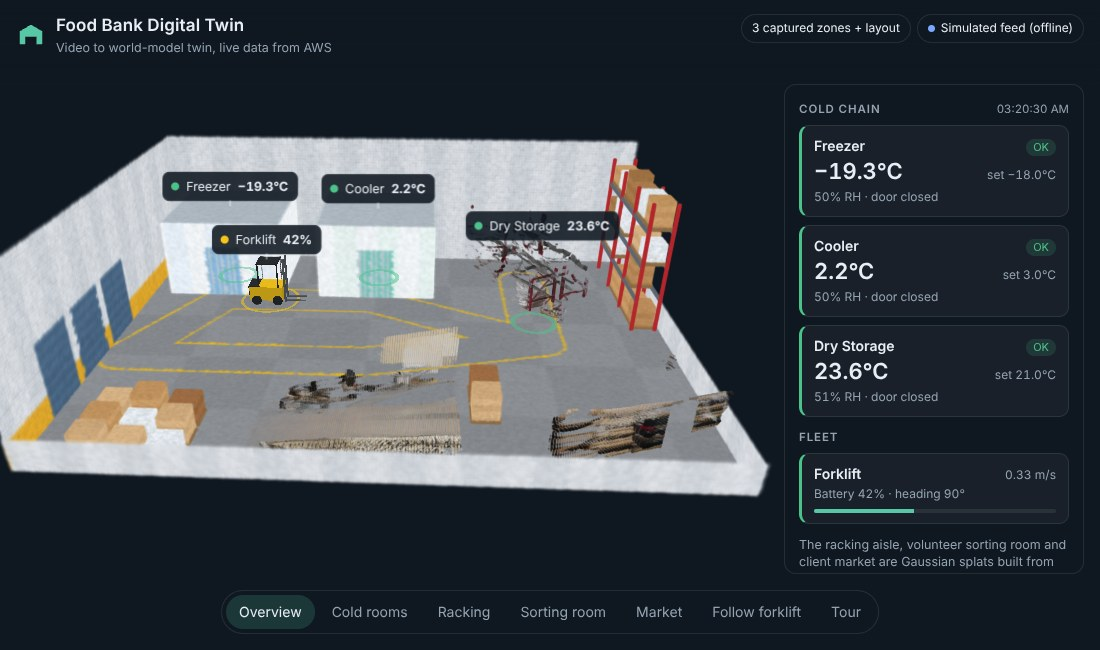
\includegraphics[width=\linewidth]{demo_overview.jpg}
  \caption{\label{fig:browserA}}
\end{subfigure}\hfill
\begin{subfigure}{0.49\textwidth}
  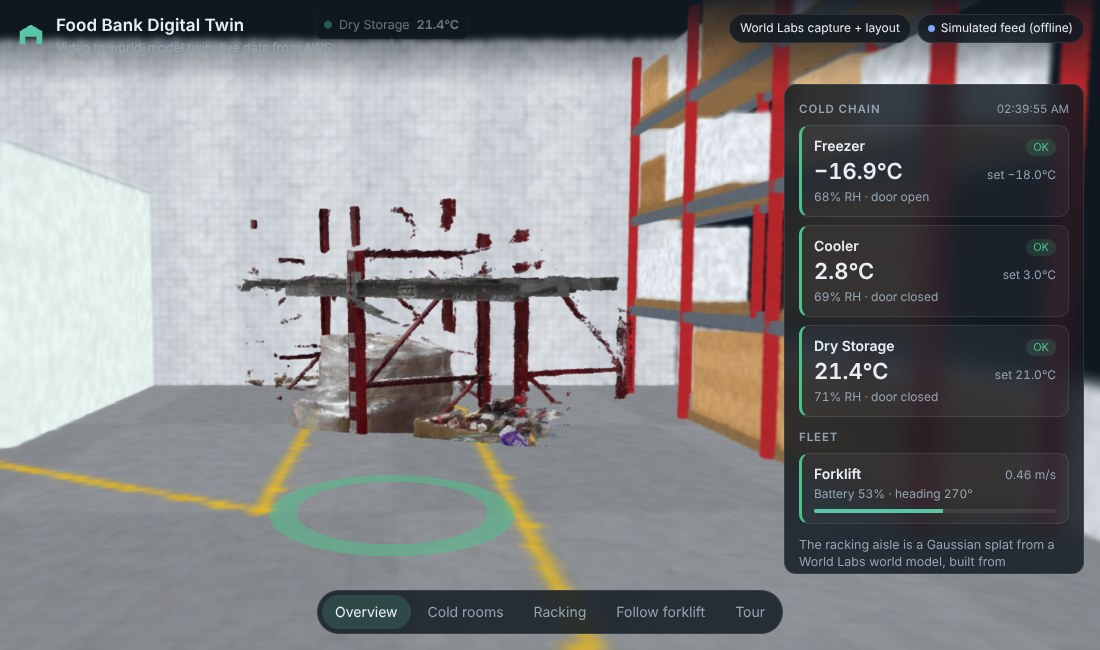
\includegraphics[width=\linewidth]{demo_aisle.jpg}
  \caption{\label{fig:browserB}}
\end{subfigure}
\caption{The browser viewer. (\subref{fig:browserA}) Overview of the three
captured zones inside the generated building, with live labels for the
freezer, cooler, dry storage and forklift and the cold-chain panel.
(\subref{fig:browserB}) The racking capture from its source viewpoint; the
red racking and pallet in the center are reconstructed, while the walls and
the racking on the right belong to the generated building.}
\label{fig:browser}
\end{figure}

\subsection{The OpenUSD stage renders outside the browser}
Two renderers read \code{site.usdz} directly on a four-core CPU machine with
no GPU, from the same list of six camera shots (Figure~\ref{fig:usdrenders}). A
Gaussian-splat renderer written for this work walks the stage for every splat
prim, applies each prim's transform to positions and covariances, and
composites the splats in depth order; it rendered all six stills in about
20\,s including loading, and a 24\,s, 576-frame 1080p flythrough in a few
minutes. Blender 5.2's own USD importer brings in the transform hierarchy but
turns each splat prim into an empty object, because it does not read the
\code{ParticleField3DGaussianSplat} schema. Reading the splats with the OpenUSD
library that ships inside Blender and drawing each as an emissive sphere gave
renders in Cycles that match the splat renderer shot for shot, at about 5\,s
per 960\,$\times$\,540 frame with 8 samples. In both, each zone reads well only
near its source viewpoints; wide shots break into fragments because the
captures are sparse, which more frames or generated views would address, not
a different renderer. \TBD{Omniverse version and hardware, confirmation that it
renders the splat schema natively, measured frame rate, and a screenshot with
telemetry overlays (Figure~\ref{fig:omniverse})}.

\begin{figure}[t]
\centering
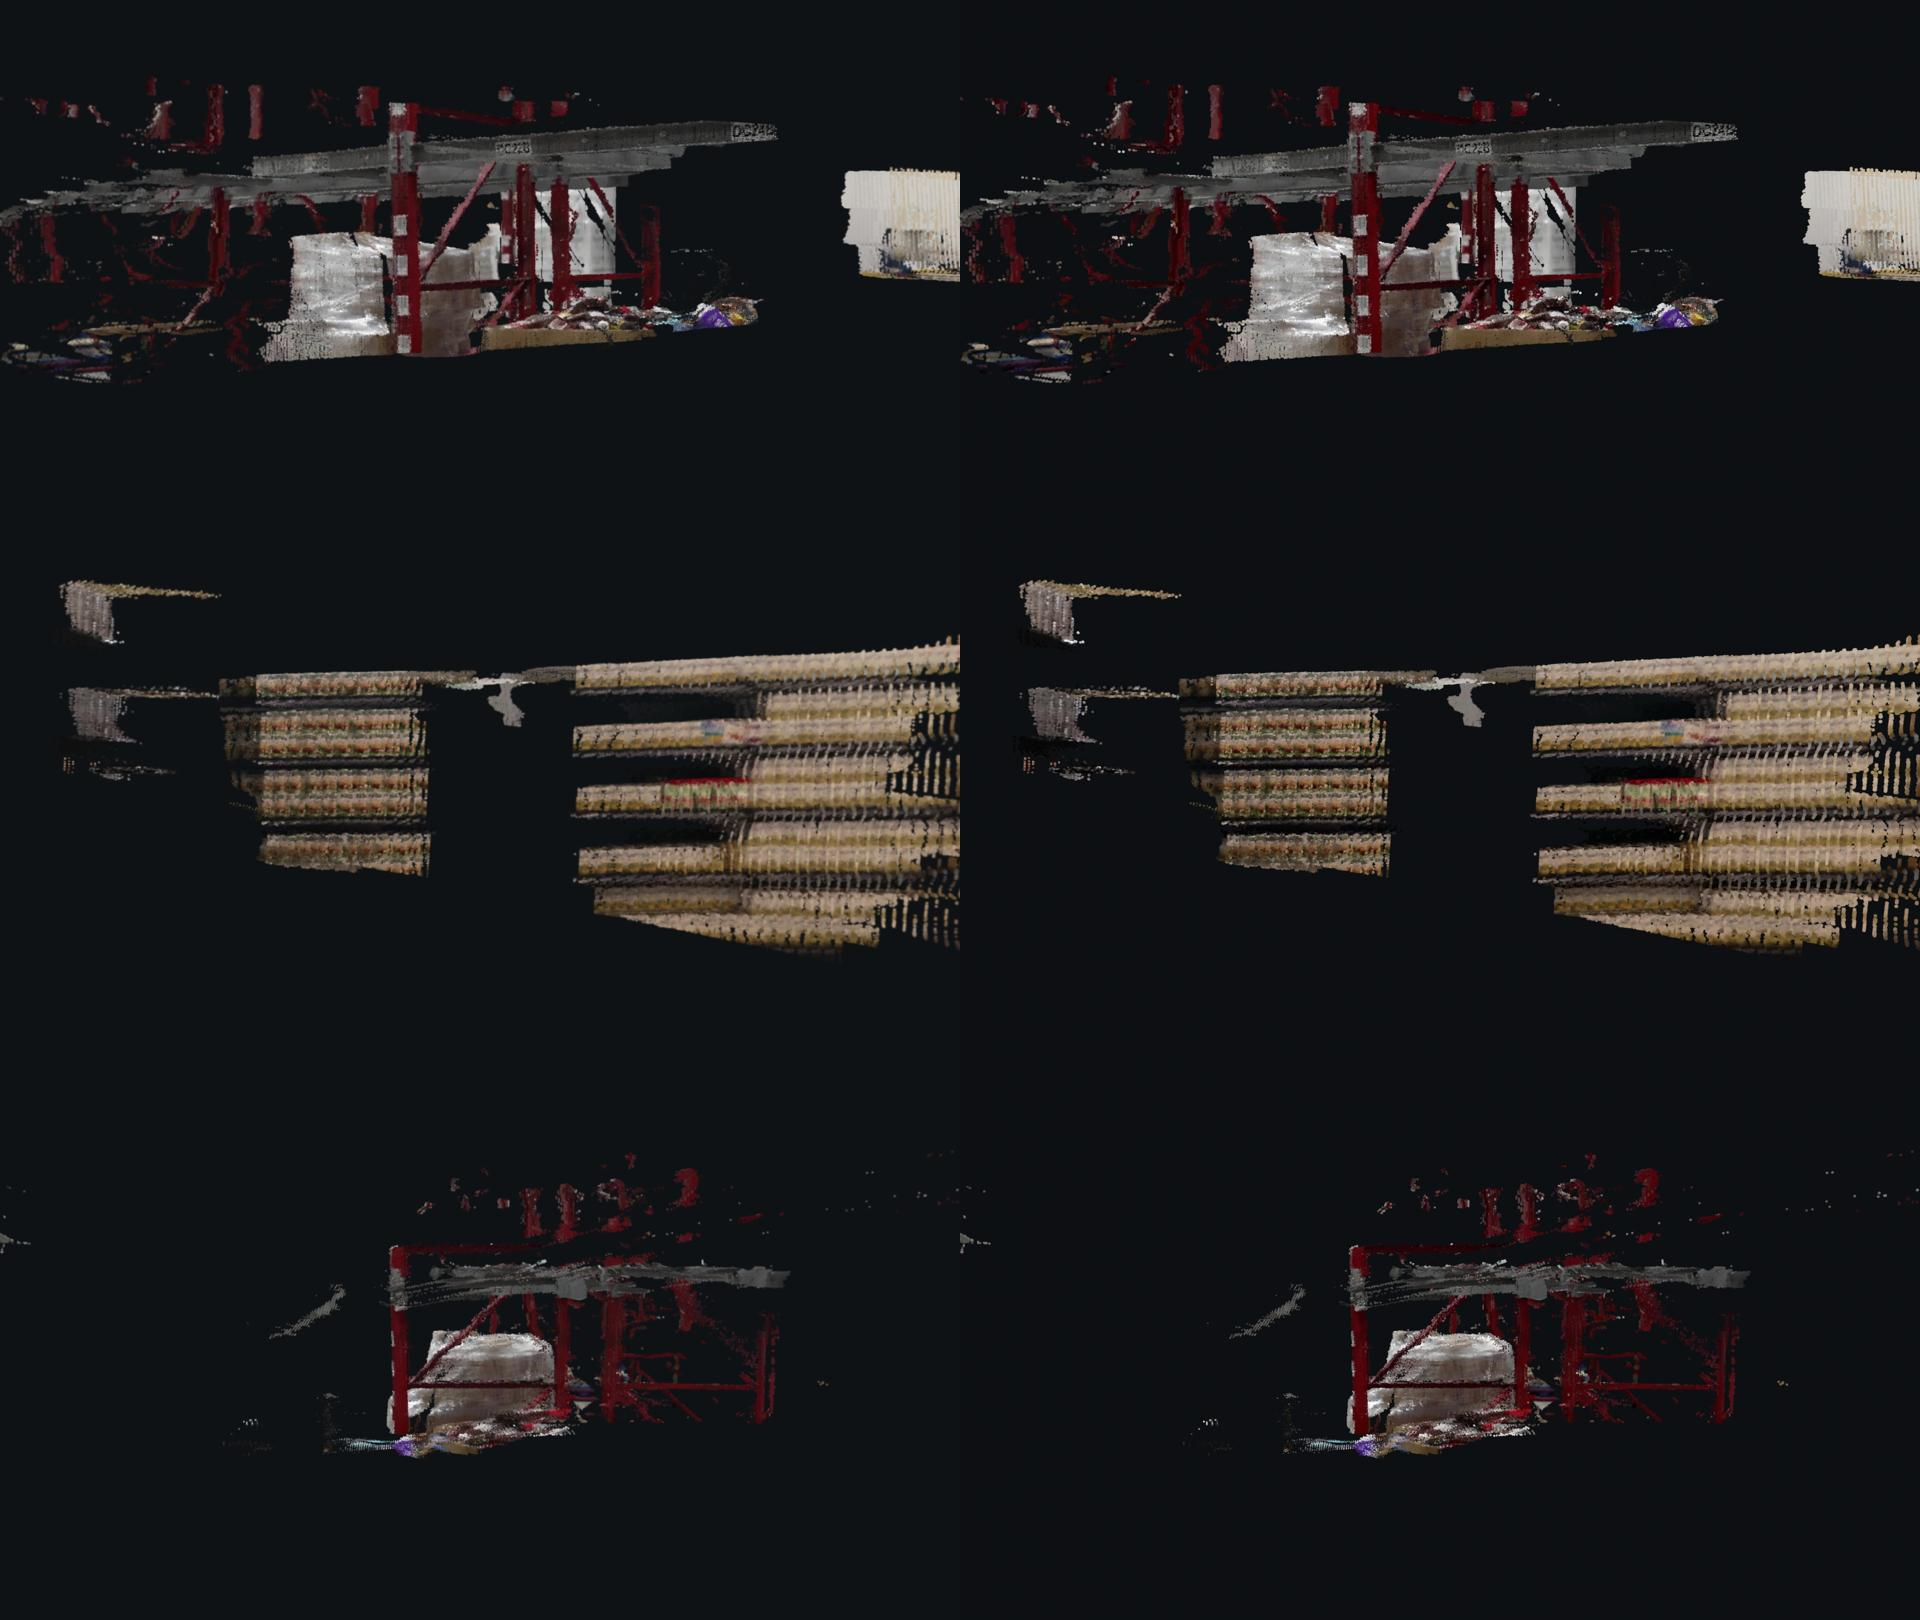
\includegraphics[width=0.8\linewidth]{splat_vs_blender.jpg}
\caption{The same OpenUSD stage rendered on a CPU, from identical cameras: the
Gaussian-splat renderer (left) and Blender 5.2 Cycles with one emissive sphere
per splat (right). Rows: the racking aisle, the client market, and the racking
aisle from an oblique viewpoint. All three shots are near the zones' source
viewpoints.}
\label{fig:usdrenders}
\end{figure}

\begin{figure}[t]
\centering
\figplaceholder{5.5cm}{Omniverse screenshot of the case-study twin with live cold-chain overlays.}
\caption{The food bank twin in NVIDIA Omniverse with telemetry bound to zone prims. \TBD{capture}}
\label{fig:omniverse}
\end{figure}

\subsection{Summary of measurements}
Table~\ref{tab:results} collects the cost, time and fidelity measurements, the
three properties that decide whether a small operator can adopt the approach.

\begin{table}[t]
\caption{Measurements for the three-zone twin. Values marked TBD are not yet measured.}
\centering\small
\begin{tabular}{@{}lll@{}}
\toprule
Quantity (unit) & Value & How measured \\
\midrule
Input frames used & 20 (8 + 6 + 6) & hand-picked from 40 per zone \\
Frame extraction, racking window (s) & 88 & wall clock, 4 CPU cores \\
World-model cost, posing (credits; USD) & 200; 0.20 & 10 credits per frame, rate card \\
World-model cost, failed generation (credits) & 0 to 800 & billing of failures unknown \\
Splats, racking / sorting / market & 270k / 282k / 195k & fused files \\
SPZ size, racking / sorting / market (MB) & 2.1 / 2.2 / 1.6 & committed files \\
USDZ size, racking / site (MB) & 17.5 / 48.5 & committed files \\
World-model generation time (min) & \TBD{measure} & operation start to completion \\
SPZ to USDZ, 270k / 182k splats (s) & 5.2 / 3.9 & wall clock, 4 cores \\
Fusion time (s) & \TBD{measure} & wall clock \\
Local 3DGS racking: frames; splats & 72; 181{,}556 & export metadata \\
Local 3DGS racking: SPZ; USDZ (MB) & 2.9; 11.9 & committed files \\
Hold-out PSNR (dB) / SSIM / LPIPS & \TBD{measure} & frames not used as input \\
Telemetry latency, p50 / p95 (ms) & \TBD{pending AWS} & client side, 1{,}000 requests \\
Monthly AWS cost (USD) & \TBD{pending AWS} & billing, demo traffic \\
Browser frame rate (fps) & \TBD{measure} & reference laptop and phone \\
Omniverse frame rate (fps) & \TBD{measure} & reference GPU \\
\bottomrule
\end{tabular}
\label{tab:results}
\end{table}

\section{Discussion}
A spatial digital twin does not have to start with a laser scanner. A short
walkthrough video, a world model and OpenUSD's native splat schema
produce a metric twin that Omniverse can render, and a serverless data layer
connects it to the systems an operator already has for almost no standing
cost. Keeping OpenUSD and a small JSON contract as the only interfaces makes
each step replaceable as world models, data platforms and renderers improve,
and lets an organization choose a renderer by hardware, cost and license
posture: OpenUSD is open source, Blender is GPL, and Omniverse combines open
components with NVIDIA-licensed runtime pieces. On a public interview video, 20 frames and
200 credits of world-model calls produced a three-zone OpenUSD twin that the
browser renders with live telemetry.

The main limitation in the current results is coverage. Twenty frames from an
interview walkthrough recover the parts of three zones the camera pointed at,
not whole rooms, and the generative step that should fill the rest failed on
the provider's side. Until it works, the browser demo surrounds the captures
with a procedural building, which is useful for explaining the twin but is not
a reconstruction. A second limitation is that generated is not measured. A world model completes
what the camera did not see. That is useful for a planning or communication
twin and unsafe if someone reads a generated aisle as the real one. Generated
regions should be marked in the stage, for example with an attribute on splats
or a separate USD layer, so renderers can show them differently.
No generated regions exist in the twin yet, so no such marking has been
implemented; the browser viewer draws its procedural building as a neutral grey
massing model so it cannot be mistaken for a capture. Scale comes from the world model's metric
estimate rather than a survey, so absolute dimensions should be checked
against at least one known measurement before the twin informs layout
decisions. People, motion blur, reflective steel and repetitive racking remain
hard inputs; masking people before reconstruction would help, and the world
model's API exposes masked inputs that we have not yet evaluated.

The twin is also a composite. Its geometry comes from a video that appears to
show the food bank's Waco hub, while its operating volumes come from published
figures for the 135{,}000\,sq\,ft Austin facility, and the building layout is
a stand-in; this is acceptable for a demonstration but must be stated wherever
the twin is shown. A related gap is technical: the operations layer uses the
browser viewer's placement of each zone, while the composed site stage still
uses an earlier site plan, so the two USD files cannot yet be referenced
together without re-composing the captures with the viewer's placements or
adding a transform per zone.

Applying the approach also needs care outside the software. Walkthrough
videos capture staff, volunteers and clients, so faces should be removed or the
space filmed when empty, and a facility's permission obtained before a
reconstruction is published. The next steps are a first real data connector,
most cheaply temperature loggers publishing over MQTT to AWS IoT Core
\cite{awsiotcore}, a person-aware frame picker, and training the locally reconstructed zones at full resolution on a GPU. The
first comparison with a conventional splat reconstruction already shows the
division of labor: the world model gives metric scale and usable geometry from
eight frames, while local training needs about nine times as many frames and a
scale assumption but delivers photorealism.

\section{Materials and Methods}

\subsection{Experimental Design}
The objective was to build a working twin of a food bank from a public video
and to measure cost, time and fidelity at each step (Table~\ref{tab:results}).
The design was fixed before any paid call: one zone first (the racking aisle,
eight frames), then two more zones with six frames each, the lowest-cost API
tasks available, and a project ceiling of 1{,}000 credits. All code, the AWS template and the input
frames are in the project repository.

\subsection{Frame extraction}
World-model APIs accept only a few images (Marble's multi-image mode accepts at
most eight with reconstruction enabled \cite{worldlabs_marble}). The ingest
stage samples a window of the video and, for every interval of $N$ seconds,
scores candidate frames with ffmpeg's blur detector and keeps the sharpest;
interlaced frames are deinterlaced only when flagged. A hard cap of 40 frames
bounds storage and upload. For the case study, frames were taken from
5:05--7:45 at one per 4\,s with the bottom 264 pixels cropped to remove the
broadcast graphic, giving 40 candidates at 1920\,$\times$\,816 in 88\,s of wall-clock time on
four CPU cores for the 160\,s window; all inputs
share one resolution, which reconstruction requires. The automatic picker
splits the pool into eight equal segments and keeps the frame with the highest
Laplacian variance in each; for the case study it was replaced by hand
selection as described in Results. A text prompt described the space and asked
for no people.

\subsection{World-model reconstruction}
The pipeline implements two routes on the World Labs platform. The first, a
multi-image request to Marble that returns a finished Gaussian-splat world in
SPZ format \cite{spz} with a metric scale factor and ground-plane offset
\cite{worldlabs_spz}, needs a Marble v1 key and was not available to the
account used here. The reported twin was built with the second route, through
the Marble 2 developer API, in three stages. In the pose stage,
\code{images2PosedRGBD} returns a camera pose, metric depth and confidence for
each input frame (10 credits per frame on the rate card of 19 October 2026,
where 1{,}000 credits cost US\$1). In the generate stage, \code{atlasGenerate}
is asked for new posed RGB-D views from target cameras around the zone, with
the masked presenters excluded from its context (50 credits per view); this is
the step in which the world model extrapolates unseen space, and it failed in
both attempts (Results). In the free, local fuse stage, every RGB-D view is
unprojected, the most confident sample per 1\,cm voxel is kept, masked pixels
are dropped, and the points are written as isotropic Gaussians with spherical
harmonics of degree 0, as PLY and SPZ version 2. The floor is taken, in order
of preference, from a dense 5\,cm horizontal slab of points, from the world
model's ground plane, or from a fixed 1.5\,m below the cameras. A site stage
then places each zone on a plan in meters (racking at the origin, sorting at
$+26$\,m and the market at $-24$\,m on $x$) and writes one USD stage that
references each zone's layer. The layout is inspired by the Central Texas Food
Bank and is not a survey.

\subsection{Locally trained zones}
The photoreal route uses no paid service. Frames from a zone's segment of the
video are extracted at 4 to 6 frames per second and 960 pixels wide. People are
masked with a DeepLab v3 segmentation model run through MediaPipe, the masks
are grown by 35 pixels and unioned with neighboring frames, and the broadcast
graphic is masked by a fixed box. Frames are kept if they are not in the
blurriest 20\%, at least 35\% of their pixels are unmasked, and the median
optical flow since the last kept frame is at least 14 pixels. COLMAP 3.9
estimates poses with masked SIFT features on the CPU. The trainer implements
3D Gaussian Splatting \cite{kerbl20233d} in plain PyTorch with a sparse
per-pixel rasterizer, so that it runs without a GPU (about 1\,s per step at
480 pixels on four cores): elliptical weighted average projection, front-to-back
compositing, an L1 plus 0.2 D-SSIM loss with masked pixels down-weighted against
a soft inpainted fill, adaptive cloning, splitting and pruning, and opacity
resets every 3{,}000 steps, at half resolution for the first quarter of the
steps. Export levels the scene to the mean camera up direction, places the
floor at the densest low slab of opaque splats, scales so that the cameras sit
1.6\,m above it, keeps splats seen by at least six cameras within 30\,m of the
path, and writes the same SPZ, USDZ and index files as the world-model zones.

\subsection{Conversion to OpenUSD}
The splat world is converted with \code{usd-convert-gsplat} 0.1.15
\cite{usdconvertgsplat} into a
\code{ParticleField3DGaussianSplat} prim.
World Labs SPZ files use an OpenCV-style camera frame (Y down) in arbitrary
units \cite{worldlabs_spz}. Leaving the splat payload untouched, we place it
under a parent transform, as shown in Equation~\ref{eq:xform},
\begin{equation} \label{eq:xform}
  M = R_x(180^\circ)\, T(0, -o, 0)\, S(s),
\end{equation}
where $s$ is the world's metric scale factor and $o$ its ground-plane offset,
and set the stage to Y-up with \code{metersPerUnit}\,=\,1. With synthetic
input the ground lands at exactly $y=0$. A typed \code{Xform} that references
the splat would override the referenced prim's schema type, so the pipeline
authors \code{/World/FoodBank} as the transforming \code{Xform} and
\code{/World/FoodBank/Splat} as an untyped prim carrying the reference. The
converter's direct USDZ output is an ASCII layer zipped without the 64-byte
alignment the USDZ specification requires, so we convert to binary
\code{.usdc} and package with OpenUSD's \code{UsdUtils.CreateNewUsdzPackage}.
Conversion took 5.2\,s for the 270{,}423-splat world-model racking zone and
3.9\,s for the 181{,}556-splat locally trained one on four CPU cores. The schema
defines half-precision attributes that would roughly halve file size; the
converter does not yet write them.

\subsection{Cost controls for paid generation}
World-model calls are the only paid, non-idempotent steps, so they are
guarded in code. On the Marble 2 route, each paid stage records its operation
identifier before waiting and sends an idempotency key derived from the request
body, so a re-run resumes or reuses a result instead of paying again; a credit
ceiling is passed per stage. The Marble v1 route adds the following guards.
Only the draft model is allowed unless explicitly overridden, and the model is
checked again in the payload and in the returned world. Each process makes at
most one billable call. The operation identifier is saved the moment a job is
accepted, so a crash resumes polling instead of paying again, and a finished
world is reused unless a new one is forced. A lifetime ledger refuses any run
that would exceed the budget, a live balance check requires a reserve, and the
billable request is retried only on HTTP 429, which the API defines as not
accepted, never on timeouts or server errors. These guards were exercised
against a local mock of the API covering a 429 retry, a 503 during polling,
resume in flight with exactly one generation across three runs, reuse,
refusal of non-draft models and ledger accounting.

\subsection{Serverless data backend}
The backend is one AWS Serverless Application Model template \cite{awssam}: an
S3 bucket serving the twin assets and web viewer; a Python 3.12 Lambda
function on arm64 with 128\,MB of memory and a 3\,s timeout behind an HTTP API
with \code{GET /telemetry} and \code{GET /health}, throttled to 5 requests per
second (burst 10) as a cost ceiling; and a log group with seven-day retention.
The telemetry function is stateless and deterministic: every value is a
function of the wall clock, so clients in the same second see the same state
without shared storage. Zone temperatures follow a slow sinusoidal drift with
a 15-minute period plus per-5-second jitter, doors open in about 10\% of
30-second windows, and alarm status is set when the deviation from setpoint
exceeds the zone's band. Responses are cacheable for 2\,s and every payload
carries \code{simulated: true}. Zone and asset anchors are in meters in the
twin frame. In the browser viewer, each capture's placement, crop box and the
area of generated geometry it replaces are set by hand in a configuration file.
The simulated zone anchors have not yet been calibrated against the captures,
so their residual error is not measured.

\subsection{Operations model}
The master data lists areas with footprints and positions in meters, six
inventory families with a home temperature zone, pallet weight, shelf life and
days-of-supply target, five inbound source types and four outbound channels
with their shares and product mixes, and the kitchen's programs, equipment,
recipes with per-meal bills of materials, and routing. Each value is either
tied to a reference or marked as an estimate. Daily inbound follows the annual
volume, a weekday profile and deterministic noise; outbound is set so stock
tracks a slow target curve, so one day's closing stock is the next day's
opening stock. Areas whose cold-chain sensor is in alarm report their stock as
at risk; the kitchen walk-in is a fourth cold-chain sensor in the telemetry
feed. Kitchen batches of 250 meals start at 06:00 local time, staggered by 45
minutes, and are dispatched between 13:00 and 15:30. Tests check that the
Python and JavaScript payloads agree, that stock carries over midnight and that
Sunday is closed. The weekday ranges in Results were computed by evaluating the
model at the end of each day from 1 September to 26 October 2026.

\subsection{Visualization}
In Omniverse, a small extension is planned that polls \code{/telemetry} and
updates prims under the twin: zone markers change color with alarm status,
labels show temperatures, and the forklift prim follows its reported position
and heading. The plan is to open the same stage on a rented RTX GPU, where
Omniverse renders particle-field prims natively, and capture the camera list
used for the CPU renders.
\TBD{Kit version and whether this is a Kit app template or a plain stage plus
extension}. The browser viewer renders the zone SPZ files with Spark
\cite{spark}, a three.js Gaussian-splat renderer, places them with the site
plan, and overlays the same telemetry; a procedural splat layout of the
building surrounds the captures and is labeled as generated. The site deploys
as static files to GitHub Pages; common USD web viewers hand USDZ to AR Quick
Look, which does not render USD particle fields. The CPU splat renderer uses
usd-core, NumPy and Numba, projects each Gaussian with an elliptical weighted
average filter, colors it from its degree-0 spherical harmonics and blends
front to back. For Blender \cite{blender}, a script reads every splat prim with
the \code{pxr} module, builds one point cloud per prim with Geometry Nodes
(radius 1.7 times the splat scale, emission color, opacity as transparency) and
renders with Cycles on the CPU; the scene can be saved as a \code{.blend} file
and explored in the Blender interface. Spheres are not Gaussians, so edges are
harder than in the splat renderer.

\subsection{Statistical Analysis}
Fidelity is measured on held-out frames: frames from the extraction window
that were not given to the world model. Their camera poses are estimated
against the reconstruction and the twin is rendered from those poses; we
report mean PSNR, SSIM and LPIPS over the held-out set with
\TBD{N held-out frames and the dispersion statistic}. Because the world model
is allowed to invent unseen content, these metrics are meaningful only in
observed regions. Latency is reported as the 50th and 95th percentiles of
1{,}000 client-side requests. \TBD{confirm protocol and pose estimation
method}.

\subsection{Animal and Human Studies}
No human subjects research was performed. The input is a publicly broadcast
news video; people who appear in it were excluded from input frames where
possible and the world model was prompted to omit them. \TBD{obtain and record
permission from the Central Texas Food Bank and the video's rights holder
before publishing renders of the reconstruction}.

\section*{Acknowledgments}

\subsection*{General}
\TBD{thank the Central Texas Food Bank and 25 News KXXV, with their
permission}. During the preparation of this work, the author used Claude
(Anthropic) in order to write and test the pipeline software and to draft the
manuscript. After using this tool, the author reviewed and edited the content
as needed and takes full responsibility for the content of the publication.

\subsection*{Author Contributions}
S. Mohapatra conceived the idea, designed the study, conducted the
experiments and wrote the manuscript.

\subsection*{Funding}
This research received no specific funding.

\subsection*{Competing interests}
The author declares that there is no conflict of interest regarding the
publication of this article.

\subsection*{Data Availability}
Code, the AWS template, the operations master data and the case-study input
frames are available at
\url{https://github.com/pikulsomesh/foodbank-spatial-twin}. The source video
is publicly available from its publisher \cite{kxxv2026ctfb}. The fused zone
files (SPZ), the composed USD site and the per-zone placements are in the same
repository; public release of renders is subject to the facility's permission.

\section*{Supplementary Materials}
Movie S1. Recorded tour of the browser twin with simulated telemetry, rendered
frame by frame in a headless browser. \TBD{replace the draft recording with the
final cut}

Movie S2. A 24\,s 1080p flythrough of the OpenUSD stage, rendered with the CPU
Gaussian-splat renderer.

Movie S3. The twin in NVIDIA Omniverse with live telemetry. \TBD{record}

Data file S1. Commands to reproduce the pipeline end to end, in three files in
the repository's \code{docs} folder: \code{CTFB\_WAREHOUSE\_RUN.md}
(world-model zones), \code{PHOTOREAL.md} (locally trained zones) and
\code{RENDERING.md} (CPU, Blender and planned Omniverse renders).

\printbibliography

\end{document}
